\documentclass[11pt]{amsart}
\usepackage[
style=apa, natbib=true,
]{biblatex}
\addbibresource{biblio.bib} 
%prepared in AMSLaTeX, under LaTeX2e
\addtolength{\oddsidemargin}{-.65in}
\addtolength{\evensidemargin}{-.65in}
\addtolength{\topmargin}{-.5in}
\addtolength{\textwidth}{1.2in}
\addtolength{\textheight}{1.0in}
\renewcommand{\baselinestretch}{1.06}

\usepackage{wrapfig,fancyvrb,xspace}
\usepackage{palatino,bm,stmaryrd}
\usepackage[final]{graphicx}
\usepackage[pdftex, colorlinks=true, plainpages=false, linkcolor=blue, citecolor=red, urlcolor=blue]{hyperref}

% macros
\newcommand{\bn}{\mathbf{n}}
\newcommand{\bq}{\mathbf{q}}
\newcommand{\bu}{\mathbf{u}}
\newcommand{\bv}{\mathbf{v}}
\newcommand{\bw}{\mathbf{w}}
\newcommand{\bx}{\mathbf{x}}

\newcommand{\bX}{\mathbf{X}}
\newcommand{\bZ}{\mathbf{Z}}

\newcommand{\bzero}{\bm{0}}

\newcommand{\bsigma}{\bm{\sigma}}
\newcommand{\bomega}{\bm{\omega}}

\newcommand{\cH}{\mathcal{H}}
\newcommand{\cK}{\mathcal{K}}
\newcommand{\cT}{\mathcal{T}}
\newcommand{\cV}{\mathcal{V}}

\newcommand{\dx}{\mathrm{dx}}
\newcommand{\ds}{\mathrm{ds}}

\newcommand{\RR}{\mathbb{R}}

\newcommand{\Div}{\nabla\cdot}
\newcommand{\eps}{\epsilon}
\newcommand{\grad}{\nabla}
\newcommand{\lam}{\lambda}

\newcommand{\jump}[1]{\llbracket #1 \rrbracket }

\newcommand{\Patm}{P_{\text{atm}}}
\newcommand{\Pbot}{P_{\text{bot}}}


\title{Gas in a porous media, using Firedrake}
\author{Tara Shreve}
\author{Ed Bueler}
\date{\today}

\begin{document}
\maketitle
%\begin{abstract}
%FIXME
%\end{abstract}

\thispagestyle{empty}

\section{Introduction}

\subsection{Porous media with Darcy-type gas flow}  Suppose $\Omega$ is a 2D or 3D domain with well-behaved boundary.  We will use $x,y$ for the horizontal coordinates and $z$ for the vertical coordinate on $\Omega$.  (In 2D we use only $x,z$.)  Note distances are measured in meters and $z$ is measured positive upward.  Within $\Omega$ we assume there is a matrix of porous material with spatially-variable porosity $\phi(x,y,z)$ and permeability $k(x,y,z)$.  Regarding (SI) units, these two fields are dimensionless and in $\text{m}^2$, respectively.  They are assumed independent of time, but they are not assumed to be smooth; we are interested in cases where they have large discontinuities.

A gas flows through the porous matrix, and we will take this gas to be ideal and isothermal.  The following are thus positive constants: $R$ is the gas constant, $T$ is the absolute temperature, and $M$ is the molar mass.  The ideal gas law says the density $\rho$ and pressure $P$ are proportional with constant $c = M/(RT)$:
\begin{equation}
\rho = c P.  \label{eq:ideal}
\end{equation}

We assume that the gas flow satisfies Darcy's law \citep{Fowler2011}.  In such a model the volumetric flux $\bq$, also called the discharge, is driven by the gradient of the gas pressure.  In the presence of gravity Darcy's law reads \citep{Collinson2012}:
\begin{equation}
\bq = - \frac{k}{\mu} \left(\grad P + \rho g \grad z\right) \label{eq:darcy}
\end{equation}
Here $\mu$ is the dynamic viscosity of the gas, again taken to be constant, $g$ is the acceleration of gravity, and $\grad z = (0,0,1)$.  

In addition to flow, we allow for the possibility that gas is generated within the domain $\Omega$.  The rate is given by a source function $Q_m(t,x,y,z)$, in units of mass per volume per time.  Because mass is conserved \citep{Tadmor2012}, the following equation holds:
\begin{equation}
\phi \frac{\partial \rho}{\partial t} + \Div \left(\rho\, \bq\right) = Q_m. \label{eq:masscont}
\end{equation}

Certain observations can already be made about equations \eqref{eq:ideal}--\eqref{eq:masscont}.  First, gas density must be non-negative: $\rho\ge 0$.  Second, relative to the classic, source-free mass continuity statement ``$\partial\rho/\partial t + \Div(\rho \bv)=0$'' \citep[equation (4.3)]{Tadmor2012}, wherein $\bv$ is the fluid velocity, note that \eqref{eq:masscont} is scaled with the porosity $\phi$.  In fact $\phi$ is implicit in the definition of $\bq$, which is the gas volume per unit area through any face of the porous matrix.  Thus $\bq = \phi \bv$ where $\bv$ is the fluid velocity.  (However, while $\bv$ may be helpful in understanding the physical problem, it is not required when stating the model.)  Third, note that a no-flow condition $\bq=\bzero$ implies, using \eqref{eq:ideal} and \eqref{eq:darcy}, the equation $\partial P/\partial z = -cg P$.  If the pressure is atmospheric ($\Patm$) at the surface $z=L$ then we find that $P(z) = \Patm \exp(cg(L-z))$, thus the no-flow pressure distribution grows exponentially with depth.  On the other hand, this distribution is \emph{not} the same as the lithostatic pressure distribution, which is generated by the weight of (deformable) rock or magma above the gas \citep[equation (5)]{Collinson2012}.  Finally, regarding units of the solution fields, $\rho(t,x,y,z)$ is in $\text{kg}\,\text{m}^{-3}$, $P(t,x,y,z)$ in $\text{Pa} = \text{N}\,\text{m}^{-2}$, and $\bq(t,x,y,z)$ in $\text{m}^3\,\text{m}^{-2}\,\text{s}^{-1} = \text{m}\,\text{s}^{-1}$.  The constant $c$ is in $\text{kg}\,\text{J}^{-1} = \text{kg}\,\text{N}^{-1}\,\text{m}^{-1}$, and the dynamic viscosity $\mu$ is in $\text{Pa}\,\text{s}$.

It is straightforward to eliminate the pressure $P$ and flux $\bq$ from the system \eqref{eq:ideal}--\eqref{eq:masscont}, yielding an evolution equation for density:
\begin{equation}
\phi \frac{\partial \rho}{\partial t} - \Div \left(\frac{k}{\mu} \left(\frac{1}{c} \rho \grad \rho + g \rho^2 \grad z\right)\right) = Q_m. \label{eq:primal}
\end{equation}
This form is comparable to the time-dependent heat equation \citep{Evans2010}:
\begin{equation}
\frac{\partial u}{\partial t} - \Div(\grad u) = 0. \qquad \text{\emph{(heat equation)}}\label{eq:heat:primal}
\end{equation}
A well-known property of \eqref{eq:heat:primal} is that the operator $\Div \grad = \grad^2$ acts as an invertible matrix when finding the solution $u$.  By contrast, since $\rho$ appears as a flux coefficient in \eqref{eq:primal}, invertibility of its corresponding operator will be lost if $\rho\to 0$ somewhere.  Such ``degeneration'' of the diffusivity is a common concern regarding the properties of the porous medium equation \eqref{eq:primal} \citep[for example]{Vazquez2007}.

Suitable boundary conditions must be applied to \eqref{eq:primal}.  On the Dirichlet portion of the boundary, denoted $\Gamma_D \subset \partial\Omega$, the density is given by a continuous function $\rho_D(x,y,z)$, or equivalently the pressure may be given.  On the remainder of the boundary $\Gamma_N = \partial\Omega \setminus \Gamma_D$, the Neumann portion, the normal mass flux may be set to zero, $\rho\bq\cdot \bn = 0$, as we will do here.  Alternatively, it is straightforward to extend the model with provided values of the mass flux, $\rho\bq\cdot \bn = \sigma_N$ where $\sigma_N$ is given, a non-homogeneous condition.

Let $\rho_0(x,y,z)=\rho(0,x,y,z)$ be an everywhere-positive, continuous initial density.  Mathematically, with these boundary and initial conditions it follows that a unique classical solution to \eqref{eq:primal} exists if in addition $k$ is smooth and $\rho_D$ is positive \citep[Theorem 3.1]{Vazquez2007}.  On the other hand, we will address weak solutions, for which $k$ need not be smooth, in the next section.

\subsection{Linearization of the diffusion}  A straightforward substitution converts nonlinear model \eqref{eq:primal}, which has nonlinear and degenerate diffusivity, into an equation which is easier to solve and which does not degenerate in the same way.  The new equation remains nonlinear, but its spatial operator is a linear, constant-coefficient operator of advection-diffusion type.  The substitution is simply
\begin{equation}
u = \rho^2. \label{eq:defu}
\end{equation}
We also define the positive constant $\alpha = 1/(2c\mu)$ and the constant vector field $\bZ=(g/\mu) \grad z=(0,0,g/\mu)$.

Considering the time-dependent problem over duration $T>0$, using the boundary and initial conditions above, equation \eqref{eq:primal} becomes the strong-form problem
\begin{subequations}
\label{eq:strongu}
\begin{align}
\phi \frac{\partial(\sqrt{u}\,)}{\partial t} - \Div\Big(k \left(\alpha\grad u + u \bZ\right)\Big) &= Q_m & &\text{on } [0,T]\times \Omega \label{eq:strongu:eqn} \\
u &= \rho_D^2 & &\text{on } [0,T]\times \Gamma_D  \label{eq:strongu:bcD} \\
-k\left(\alpha\grad u + u \bZ\right) \cdot \bn &= 0 & &\text{on } [0,T]\times \Gamma_N  \label{eq:strongu:bcN} \\
u\big|_{t=0} &= \rho_0^2 & &\text{on } \Omega  \label{eq:strongu:initial}
\end{align}
\end{subequations}

Observe that the spatial derivative term now corresponds to a linear operator:
\begin{equation}
L u = - \Div\Big(k \left(\alpha\grad u + u \bZ\right)\Big).
\end{equation}
The operator is uniformly elliptic if $k$ is bounded and has a positive lower bound: $k \ge k_0 > 0$.  While \eqref{eq:strongu:eqn} is nonlinear in the time derivative, so that implicit time discretization will generate a nonlinear problem to solve at each step, because the spatial operator is linear the nonlinearity in \eqref{eq:strongu:eqn} is zeroth-order in space, and only modifies the diagonal of the Jacobian in a Newton iteration, for example.

In the steady-state case system \eqref{eq:strongu} is actually linear, and furthermore the porosity has no direct effect on the solution:
\begin{subequations}
\label{eq:sstrongu}
\begin{align}
- \Div\Big(k \left(\alpha\grad u + u \bZ\right)\Big) &= Q_m & &\text{on } \Omega \label{eq:sstrongu:eqn} \\
u &= \rho_D^2 & &\text{on } \Gamma_D  \label{eq:sstrongu:bcD} \\
-k\left(\alpha\grad u + u \bZ\right) \cdot \bn &= 0 & &\text{on } \Gamma_N  \label{eq:sstrongu:bcN}
\end{align}
\end{subequations}
Model \eqref{eq:sstrongu} is a steady-state, linear diffusion problem for the squared density $u$.  From a solution to either \eqref{eq:strongu} or \eqref{eq:sstrongu}, the density $\rho$ and pressure $P$ are easily recovered via equations \eqref{eq:ideal} and \eqref{eq:defu}, as long as the solution satisfies $u\ge 0$.

\subsection{Exact solutions useful for verification}  If they can be found and implemented easily, exact solutions of the above systems are useful tools for confirming code correctness.  One such solution has already been mentioned, the gravity-balanced, no-flow solution which is exponential in depth.  Another solution is given below, a steady-state, one-dimensional solution for piecewise-constant permeability.  We describe these solutions in sufficient detail so that they can be used as verification and regression tests.

\begin{itemize}
\item \textbf{No-flow solution.}  Consider the steady-state system \eqref{eq:sstrongu} on a rectangular domain
\begin{equation}
\Omega = [0,L_x]\times [-L_z,0] = \{(x,z)\,:\,0<x<L_x, \,-L_z<z<0\}
\end{equation}
like that shown in Figure \ref{fig:COMSOLresults}.  Suppose the pressure is atmospheric $P=\Patm$ at the upper surface $\Gamma_D=\{z=0\}$, and that zero normal flow is imposed on \emph{all} of the remaining boundary.  (The bottom pressure condition shown in the Figure is not applied.)  Thus we set $u=c^2\Patm^2$ on $\Gamma_D$ (condition \eqref{eq:sstrongu:bcD}), while \eqref{eq:sstrongu:bcN} applies on all remaining boundary $\Gamma_N$.  As one may confirm by substitution, the formula
\begin{equation}
u(x,y,z) = c^2 \Patm^2 e^{-2cgz} \label{eq:noflow}
\end{equation}
satisfies condition \eqref{eq:sstrongu:bcD}, and in fact it gives $\bq = -k (\alpha\grad u + u \bZ) = \bzero$ identically in the domain, so \eqref{eq:sstrongu:eqn} is satisfied with $Q_m=0$, and also \eqref{eq:sstrongu:bcN} is satisfied.  By uniqueness this is the solution to the boundary value problem.  Noting that the distribution of permeability is irrelevant to this construction, this solution can be used as a part of verification for any permeabilility distribution $k$.

\item \textbf{Three horizontal units solution.}  Again consider a rectangular domain as in Figure \ref{fig:COMSOLresults}, with boundary conditions as shown.  However, suppose the textural units are simplified to a permeability profile $k$ which is independent of $x$.  Specifically, assume $k$ is a function of $z$ on $[-L_z,0]$ with transition locations $z_1$, $z_2$:
\begin{equation}
k(z) = \begin{cases} k_1, & -L_z < z < z_1 \\
                     k_2, & z_1 < z < z_2 \\
                     k_3, & z_2 < z < 0. \end{cases}
\end{equation}
(No choice of the exact permeabilities at the interfaces needs to be made because the weak form, below, only sees integrals of $k$.)  Taking no mass source or gravity, $Q_m=0$ and $g=0$, and imposing pressures $\Pbot$ at $z=-L_z$ and $\Patm$ at $z=0$, symmetry implies that the solution is a function of $z$ only, and further that $u_{zz}=0$ within each textural unit.  Thus the solution of \eqref{eq:sstrongu} is a continuous and piecewise-linear function which connects the Dirichlet conditions at the bottom and top of the domain, and which has zero jump in the normal fluxes at the interfaces between units.  It has the following piecewise-defined form:
\begin{equation}
u(z) = \begin{cases} a_1 (z + L_z) + c^2 \Pbot^2, & -L_z < z < z_1 \\
                     a_2 (z - z_1) + b_2, & z_1 < z < z_2 \\
                     a_3 z + c^2 \Patm^2, & z_2 < z < 0 \end{cases} \label{eq:threehor}
\end{equation}
The constants satisfy equations stating that neither $u$ nor $k u_z$ has a jump at the unit interfaces $z=z_1,z_2$:
\begin{align}
a_1 (z_1+L_z) + c^2 \Pbot^2 &= b_2 \label{eq:threehor:linsysconstants} \\
a_2 (z_2-z_1) + b_2 &= a_3 z_2 + c^2 \Patm^2 \notag \\
k_1 a_1 &= k_2 a_2 \notag \\
k_2 a_2 &= k_3 a_3 \notag
\end{align}
The numerical solution $a_1,a_2,a_3,b_2$ of this  $4\times 4$, invertible linear system is easily found.
\end{itemize}

These two exact solutions are implemented as regression tests for the code \texttt{uporous.py}, documented below.  Convergence to these exact solutions can be confirmed, but they are too simple to allow measurement of a typical convergence rate in general circumstances.  It may be worthwhile constructing a more complicated 2D exact solution at a later time.


\section{Weak form and finite element method}

\subsection{Weak form suitable for discontinuous permeability}  Now we derive the weak form of steady-state problem \eqref{eq:sstrongu}.\footnote{The weak form for an (implicit) time-stepping solution of \eqref{eq:strongu} is a reasonably straightforward modification of the result here.  This is among our planned next steps.}  This weak form is needed for our finite element (FE) method, which will follow a standard approach often used for Poisson equations.  The method is conforming \citep{Elman2014}; it finds a continuous approximate solution in the same function space where the exact solution lives.  Both the continuum and FE solutions solve the same weak form, but the latter is over a finite-dimensional subspace.

As is common in these derivations, let $H^1(\Omega)$ denote the Sobolev (Hilbert) space of functions on $\Omega$ with weak derivatives which are square-integrable functions \citep[chapter 5]{Evans2010}, and let $H_0^1(\Omega)$ denote the subspace of functions with zero trace along $\Gamma_D$.  Supposing the strong form problem \eqref{eq:sstrongu} has a solution of some kind, we multiply equation \eqref{eq:sstrongu:eqn} by a test function $v \in H_0^1(\Omega)$.  Integration by parts\footnote{Integration by parts combines two facts.  First, for a scalar function $f$ and a vector field $\bX$, the product rule says $\Div(f\bX) = \grad f \cdot \bX + f \Div \bX$.  Second, the divergence theorem states $\int_\Omega \Div (f\bX)\,\dx = \int_{\partial \Omega} f\bX\cdot \bn\,\ds$.  These combine to $-\int_\Omega (\Div \bX) f = \int_\Omega \bX \cdot \grad f - \int_{\partial\Omega} f \bX\cdot\bn\ds$, as used here.} then generates
\begin{equation}
\int_\Omega k \left(\alpha\grad u + u\bZ\right) \cdot \grad v\,\dx - \int_{\partial\Omega} k v \left(\alpha\grad u + u\bZ\right) \cdot \bn\,\ds = \int_\Omega Q_m v\,\dx \label{eq:weaku:early}
\end{equation}
Since $v\in H_0^1(\Omega)$, the $\Gamma_D$ portion of the boundary integral in \eqref{eq:weaku:early} is zero.  Then \eqref{eq:sstrongu:bcN} implies that the remaining integral over $\Gamma_N$ is zero.  Thus the weak form is simply
\begin{equation}
\int_\Omega k \left(\alpha\grad u + u\bZ\right) \cdot \grad v\,\dx = \int_\Omega Q_m v\,\dx. \label{eq:weaku}
\end{equation}

Because we will solve cases where the permeability field $k$ has discontinuous jumps, it is worth considering the theoretical setting for \eqref{eq:weaku}.  First assume that $k\in L^\infty(\Omega)$ with a positive lower bound; there is $k_0>0$ so that $k \ge k_0$.  Such a lower bound implies that the linear operator $L w = - \Div(k \left(\alpha\grad w + w\bZ\right))$ is uniformly elliptic \citep[section 6.1]{Evans2010}.  We will assume that the boundary value $u_D = \rho_D^2$, defined only on $\Gamma_D$, is the trace of some $g\in H^1(\Omega)$, so that if $u\in H^1(\Omega)$ then $\tilde u = u - g \in H_0^1(\Omega)$.  The theory of problem \eqref{eq:weaku} then shows that there is a unique weak solution $u\in H^1(\Omega)$.  To show this, apply Theorem 3 in section 6.2 of \citep{Evans2010}, noting the comments on pages 315 and 322 regarding boundary values and the constant in the Poincare inequality, respectively.

It is the weak solution of \eqref{eq:weaku} which we are seeking to approximate in the FE method below.  The earlier strong form \eqref{eq:sstrongu} generally will not have a solution for which the stated second derivative is actually meaningful.  On the other hand, while the permeability field $k(x,y,z)$ may be discontinuous, when applying the FE method we can in many cases arrange that the element faces (edges in 2D) include all of these discontinuities.  In other words, we can often adapt the mesh to the permeability discontinuities.  In that case one can show, by integrating over each domains where $k$ is smooth, that weak form \eqref{eq:weaku} corresponds to (correctly) taking the jump integrals, which otherwise must be set, to be zero.\footnote{If needed, the details could be spelled out here.  However, a reference example is on the Firedrake documentation page \href{https://www.firedrakeproject.org/demos/immersed_fem.py.html}{\texttt{www.firedrakeproject.org/demos/immersed\_fem.py.html}}.}  Furthermore the numerical error measured for the discontinuous-$k$ verification case in the previous section is greatly reduced when the mesh is adapted to the discontinuities.

%\subsection{Finite element method}  Next we assume that the mesh (triangulation) $\cT_h$ exactly covers the domain: $\bigcup_{E\in\cT_h} \bar E = \bar \Omega$.


\section{Firedrake implementation and solution}

To implement the weak form in Firedrake we must choose a finite element space for $u$, which we take to be a space of continuous, piecewise-polynomial functions of degree $j$, namely $\text{CG}_j$ \citep{Elman2014}
\begin{Verbatim}[fontsize=\small,frame=lines]
H = FunctionSpace(mesh, 'CG', j)
u = Function(H)
v = TestFunction(H)
\end{Verbatim}
Weak form \eqref{eq:weaku} then corresponds to the UFL code
\begin{Verbatim}[fontsize=\small,frame=lines]
c = M / (R * T)
alf = 1.0 / (2.0 * c * mu)
Z = Constant(as_vector([0.0, 0.0, args.g / mu]))
F = k * dot(alf * grad(u) + u * Z, grad(v)) * dx(degree=4)
\end{Verbatim}
The quadrature degree is fixed so as to disable Firedrake's automatic quadrature degree mechanism, which can generate unstable and inefficient degrees which are too large.

Next, on $\Gamma_D$ we impose the essential requirement that $u=\rho_D^2$, and $v=0$ for the test functions, via Firedrake's \verb|DirichletBC()| command.  For example, in the case of a 3D extruded mesh with given pressure on top ($\Patm$) and bottom ($\Pbot$):
\begin{Verbatim}[fontsize=\small,frame=lines]
u_top = (c * Patm)**2
u_bot = (c * Pbot)**2
bcs = [DirichletBC(H, u_bot, 'bottom'),
       DirichletBC(H, u_top, 'top')]
\end{Verbatim}

We solve the steady-state discretized equations, a linear system,\footnote{A next step is to implement a time-stepping implicit method for \eqref{eq:strongu}.  The weak-form equations for each time step will be nonlinear, but straightforward application of Newton's method, \texttt{-snes\_type newtonls}, should work fine.} by a sparse direct matrix method \citep{Amestoy2001}:
\begin{Verbatim}[fontsize=\small,frame=lines]
solve(F == 0, u, bcs=[BCs,],
      solver_parameters = {'snes_type': 'ksponly',
                           'ksp_type': 'preonly',
                           'pc_type': 'lu',
                           'pc_factor_mat_solver_type': 'mumps'})
\end{Verbatim}
A more advanced iterative, block-wise, and multigrid solver is possible \citep[e.g.][]{Bueler2021}, but it will require careful development.


\section{An application for gas flow through a porous lava dome}

In \cite{Graham2023}, we measure permeability of samples from various textural units of the Obsidian dome and South Deadman dome using field and lab permeameters. These two domes are silicic lava flows in the Inyo Craters portion of the Mono-Inyo Craters in eastern California, a chain of silicic lava flows, domes, and explosion craters that stretches 12 km (7.5 miles) to the north-northeast of Long Valley Caldera. The Inyo craters erupted as recently as ~675 years (~1350 A.D.) before present. Prior studies subdivided the majority of the lava erupted at the Inyo Craters according to the observed vesicle textures found in different parts of each flow, subdivided coarsely vesicular pumice (CV; permeability $k_1$), dense obsidian (OB; $k_2$), and finely vesicular pumice (FV; $k_3$).  Shallow scientific bore hole drilling in the 1970's confirmed the presence of an underground magmatic intrusion, which was the source of the domes. This drilling also provided some general constraints on the depth of each distinct textural unit within the dome; see Table \ref{tab:UnitPermPoro} below.

In this study, we wish to put constraints on the surface gas flux for each textural unit at Obsidian Dome. The unit mapping of the dome is shown in Figure \ref{fig:unitMapping}, and an example cross-section is shown in Figure \ref{fig:crossSection}.  Using constraints on dome height, the depth and permeability of each unit, and assuming the dominant portion of gas is sourced from degassing of the underlying feeder dike, we can use Darcy's law to calculate the surface gas flux through each unit. This was done in \cite{Graham2023} using a 1D model of Darcy's law, as implemented in \cite{Edmonds2003}, giving the percentages shown in Figure \ref{fig:crossSection}.  The percentages are for each lithologic unit relative to the total gas flux calculated for all units, and they do not consider additional degassing that occurs through conduit processes, fractures, tuffisite veins, or porous pathways that are too large to measure.

\begin{figure}
   \centering
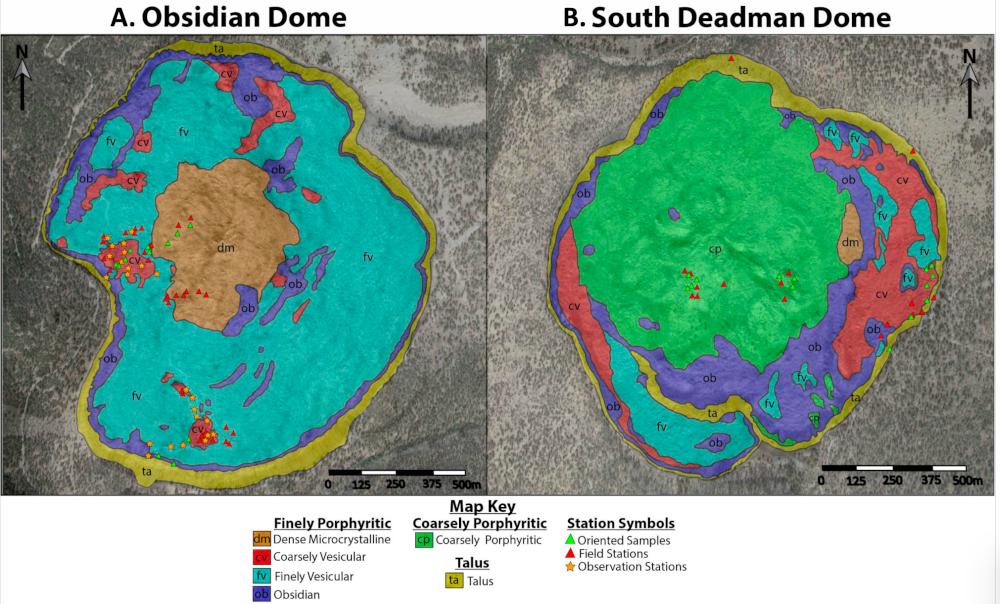
\includegraphics[width=0.9\textwidth]{figs/unitMapping-small.png}
\caption{Textural lithologic distribution maps of lavas for (A) Obsidian dome and (B) South Deadman dome.}
\label{fig:unitMapping}
\end{figure}

\begin{figure}
   \centering
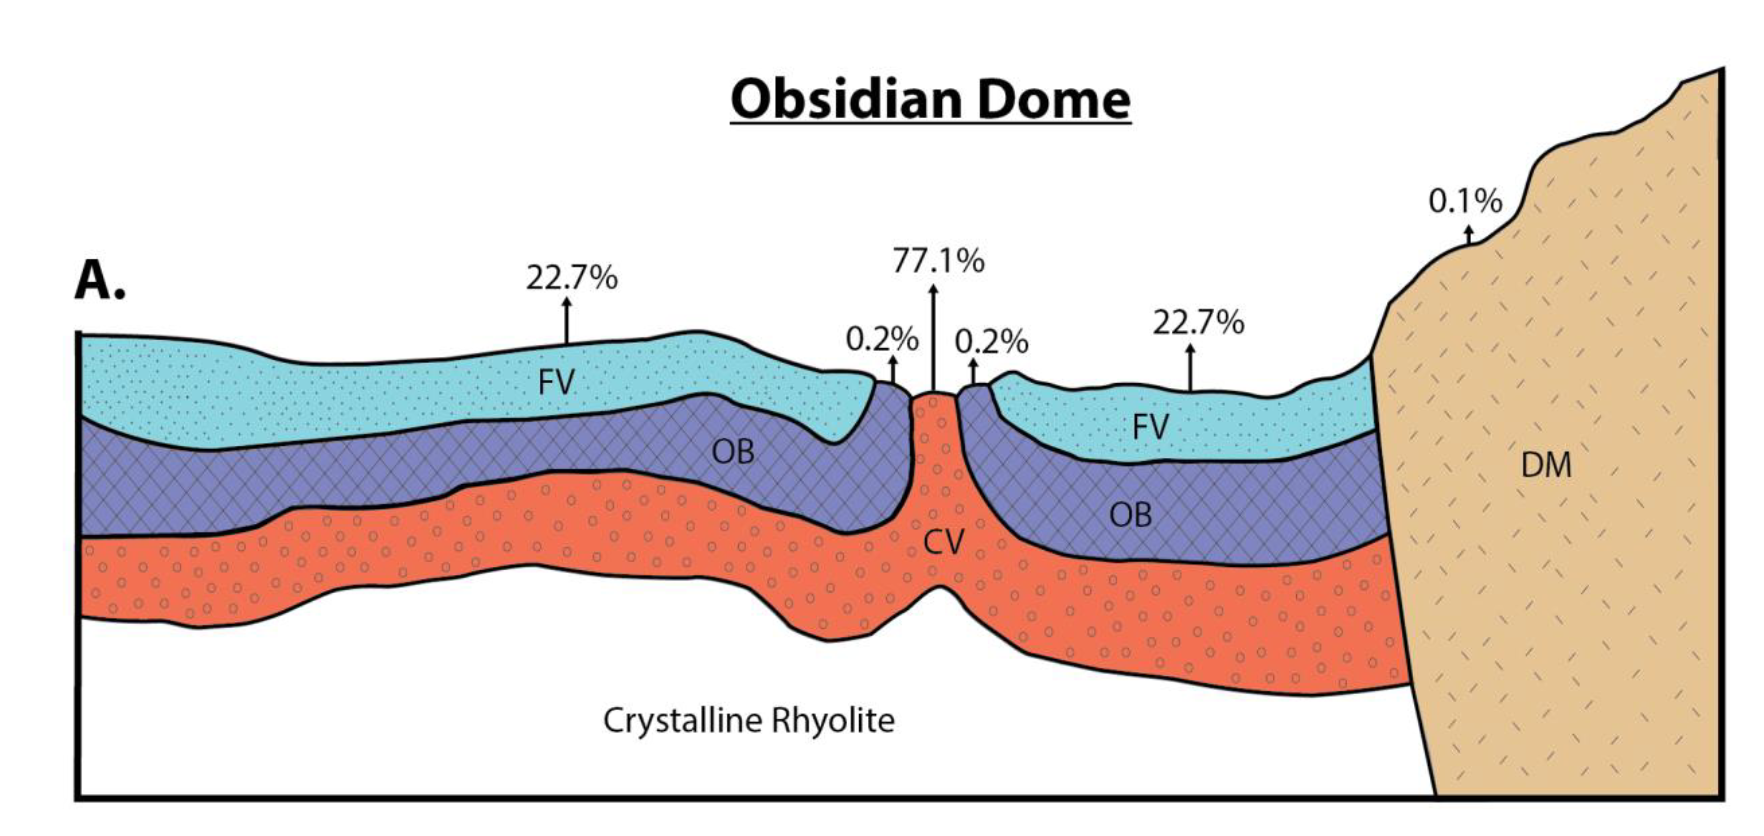
\includegraphics[width=0.9\textwidth]{figs/crossSection.png}
\caption{Schematic diagrams depicting total calculated gas flux percentages during the final stages of lava emplacement at Obsidian dome \citep{Graham2023}.  Total gas flux for each lithologic unit was calculated using the gas flux model of \cite{Edmonds2003}.}
\label{fig:crossSection}
\end{figure}

We wish to extend this model into 2D, and also 3d, to account for the unit layering and geometry, which may affect the path of gas flow towards the surface.  For initial calculations we will assume atmospheric pressure at the surface ($P_{atm} = 1.01325$ bar) and a pressure at the base of the dome ($L_z=22$ m) of $P_{z=-L_z} = 11$ bar.  There is a gas inlet at the base of the CV unit.  For simplicity, a no flow condition is imposed at the sides, and we solve for the steady-state, compressible gas flow using Darcy's Law to relate volumetric gas flux and pressure, as described above.  Also for simplicity, isothermal conditions are assumed, with steam at a temperature of 920$^{\circ}$C.  The porosity and permeability for each unit, as well as their height and percent of total dome surface area, are shown in Table \ref{tab:UnitPermPoro}.

\begin{table}[h]
\center
      \small
      \begin{tabular}{lllll}
      \hline
      \textbf{Unit} & \textbf{Permeability (m\textsuperscript{2})} & \textbf{Connected porosity (\%)}  & \textbf{Height (m)} & \textbf{Percent of total dome surface area} \\  
      \hline
      CV & 6.87E-12 & 50.0 & 10 & 6.4 \\
      FV & 2.18E-13 & 23.2 &  7 & 74.6 \\
      OB & 4.94E-15 & 3.24 & 5 & 19.0 \\ 
\end{tabular}%}
\caption{Average permeability, porosity, height, and percent of total dome surface area of each textural unit.} 
\label{tab:UnitPermPoro}
\end{table}

Earlier COMSOL model results for gas density and surface gas flux are shown in Figure \ref{fig:COMSOLresults}, with annotations stating relevant boundary conditions.  

\begin{figure}
   \centering
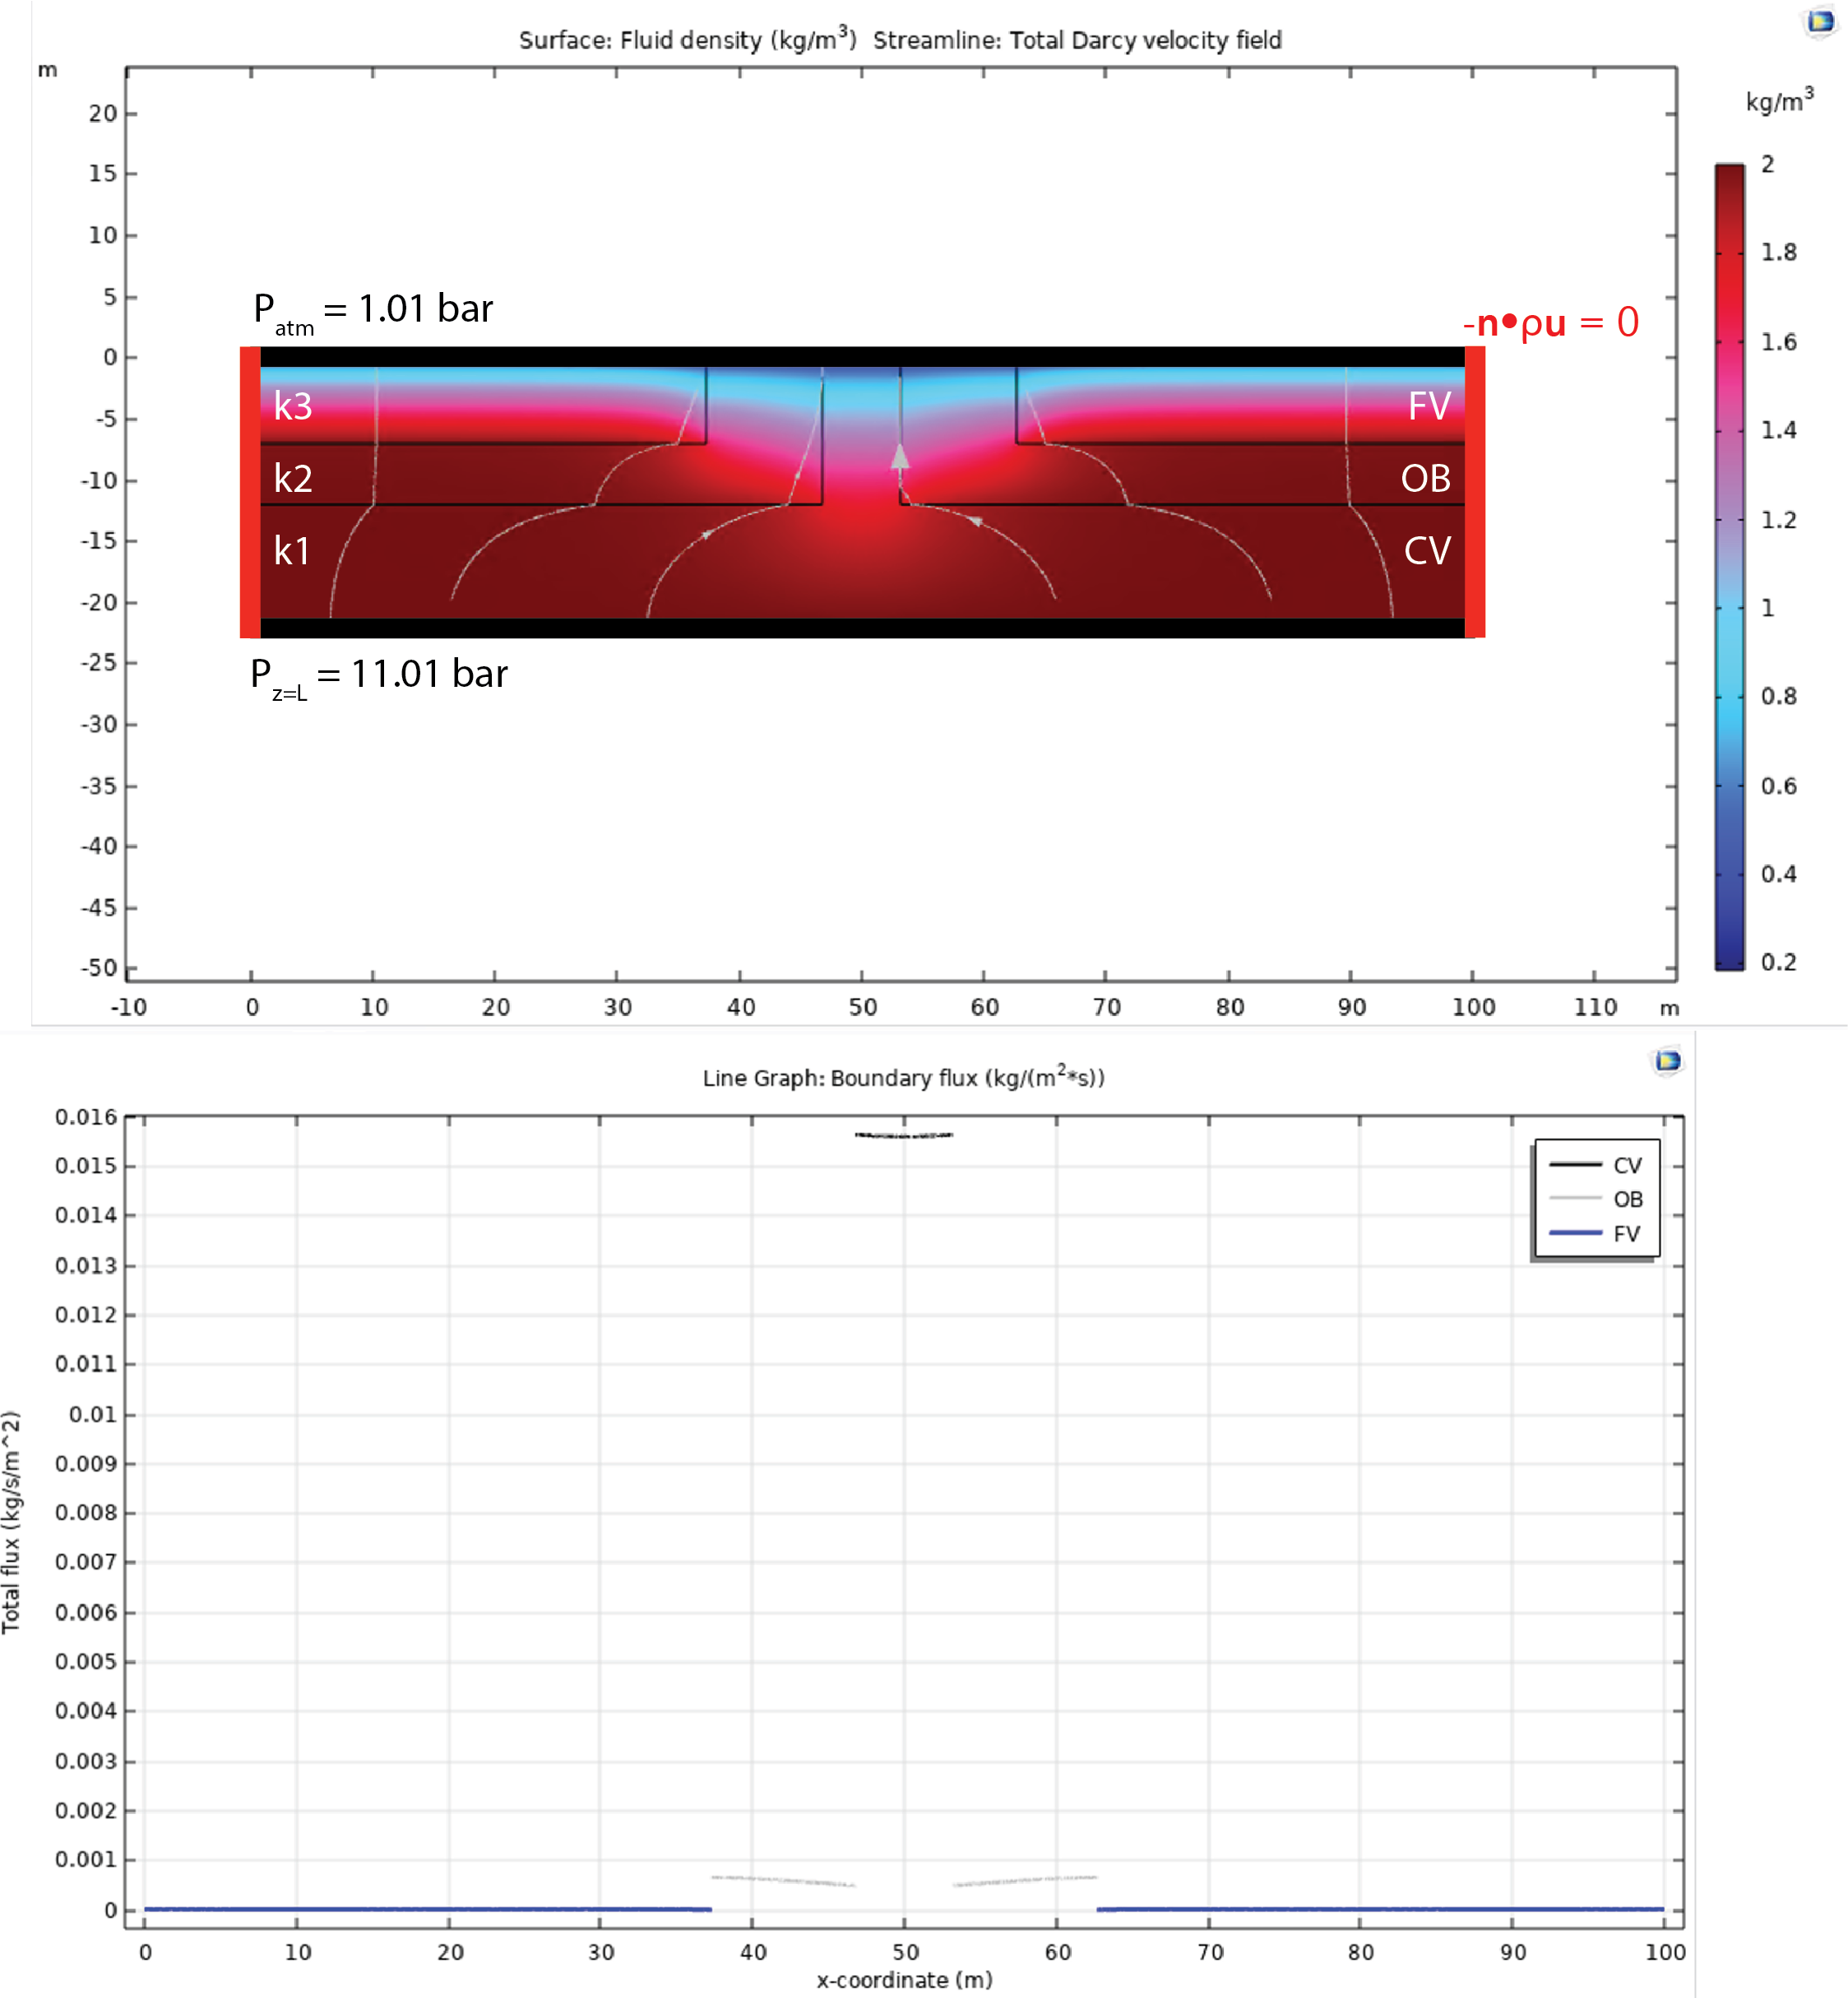
\includegraphics[width=0.9\textwidth]{figs/comsolDarcyLaw_units.png}
\caption{Top: COMSOL results for gas density in unit layers CV, FV, and OB.  Streamlines indicate the direction of gas flow.  Bottom: Gas flux at the surface, from the same computation.}
\label{fig:COMSOLresults}
\end{figure}

The Firedrake model described in earlier sections generates the somewhat different results show in figure \ref{fig:results2d}.  The following is a representative run using $CG_2$ elements on a $200\times 44$ quadrilateral mesh, which is aligned to the unit boundaries:
\begin{Verbatim}[fontsize=\small,frame=lines]
python3 uporous.py -order 2 -mx 200 -mz 44
generating 2d quadrilateral mesh of 200 x 44 elements ...
solving primal CG2 weak form for u ...
mass conservation (kg m-2 s-1):
  flux out of top         =  3.420282e-01
  flux into bottom        =  3.420282e-01
  imbalance               =  4.078127e-12
mass flux (kg m-2 s-1) for each surface unit:
  CV unit flux            =  3.337293e-01 (97.57 %)
  OB unit flux            =  3.089467e-04 ( 0.09 %)
  FV unit flux            =  7.989902e-03 ( 2.34 %)
saving fields to result.pvd ...
\end{Verbatim}

\begin{figure}
   \centering
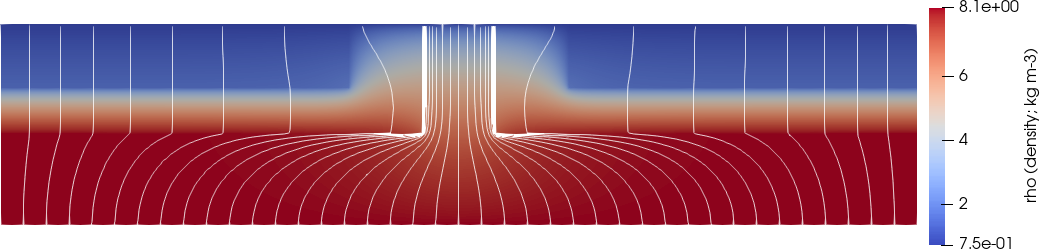
\includegraphics[width=0.9\textwidth]{figs/results2d.png}
\caption{Firedrake results showing gas density (color) and streamlines for direction of flow.}
\label{fig:results2d}
\end{figure}

The results in Figure \ref{fig:results2d} are somewhat different from those in Figure \ref{fig:COMSOLresults}.  In particular, streamlines in Figure \ref{fig:results2d} are essentially straight in the two upper units.  This would make sense in that, unlike the gas flowing out through the ``easy'' route to the CV surface unit, the gas that is in the low-permeability OB unit, or has already passed through it, will head straight for the surface.

However, if we flip the values of the permeabilities in the OB and FV units, i.e.~$k_2 \leftrightarrow k_3$, then the Firedrake results would seem to be identical to the COMSOL results,\footnote{\emph{Tara:  So this is my diagnosis for what the difference is.  For now I think Figure \ref{fig:results2d} is correct.  Can you check if you swapped values?}} as shown in Figure \ref{fig:results2dflip}.

\begin{figure}
   \centering
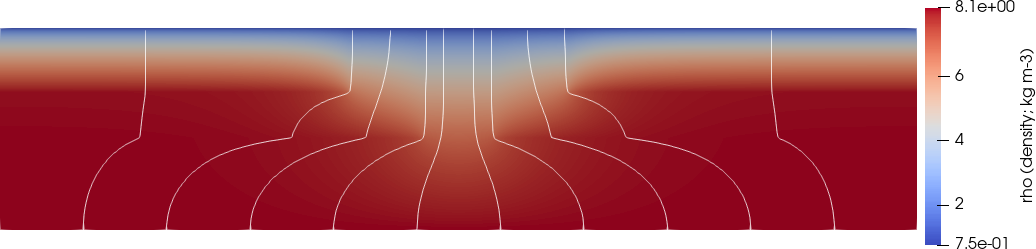
\includegraphics[width=0.9\textwidth]{figs/results2d-flipOBFV.png}
\caption{Firedrake results when we flip $k_2\leftrightarrow k_3$.}
\label{fig:results2dflip}
\end{figure}

Finally, preliminary code allows the 2D surface elevation to be read.  This can then be used to extrude a mesh in 3D.  An example is shown in Figure \ref{fig:mesh3d}.

\begin{figure}
   \centering
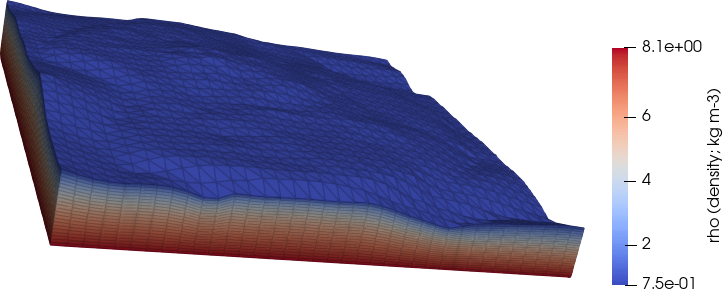
\includegraphics[width=0.7\textwidth]{figs/mesh3d.png}
\caption{Extruded 3D mesh for Obsidian Dome surface topography.  The density corresponds to constant $k$, and can be ignored.}
\label{fig:mesh3d}
\end{figure}

\printbibliography

\end{document}
